\section{Results}
\label{sec:results}

\subsection{Training Behaviour}

The training and test loss curves decrease for all eight configurations, as illustrated schematically in Figure \ref{fig:loss_curves}. The curves labelled \enquote{test} in the generated plots correspond to the test model-selection split defined above.
The selected checkpoint occurs at epoch $953$ for the velocity-only MLP and at epoch $947$ for the all-parameter MLP. For the GRUs, the selected epochs are $413$, $159$, $343$, $251$, $399$, and $390$ for configurations 03--08, respectively.
Because the objectives contain different numbers and types of standardized outputs, especially for the endpoint models in Eq. \eqref{eq:endpoint_loss}, absolute loss values should not be compared directly across every configuration.

% \begin{figure}[htbp]
%     \centering
%     % \includegraphics[width=\linewidth]{figures/loss_curves_overview.pdf}
%     \fbox{\rule{0pt}{0.22\linewidth}\rule{0.92\linewidth}{0pt}}
%     \caption{Training and test loss as a function of epoch. The log--log representation makes both the rapid initial decrease and later convergence visible.}
%     \label{fig:loss_curves}
% \end{figure}

\begin{figure}[t]
  \centering

  \subfloat[\label{fig:loss_curve_02}]{
    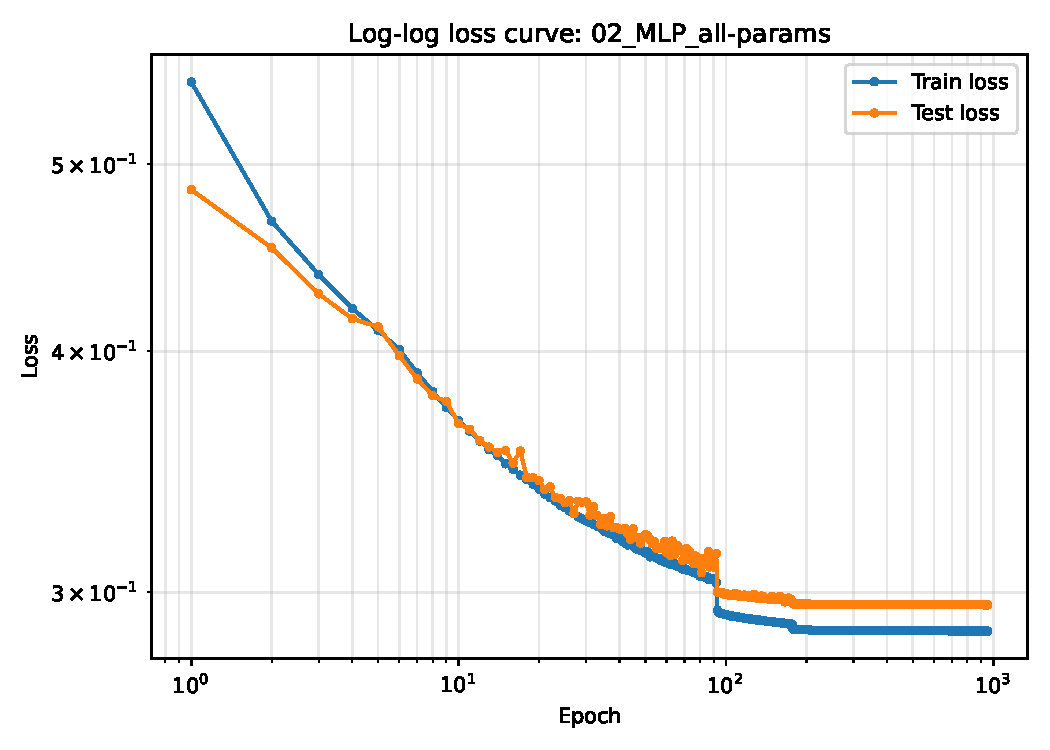
\includegraphics[width=\linewidth]{../figures/02_MLP_all-params_loss_curve_loglog}
  }

  \vspace{0.5em}

  \subfloat[\label{fig:loss_curve_05}]{
    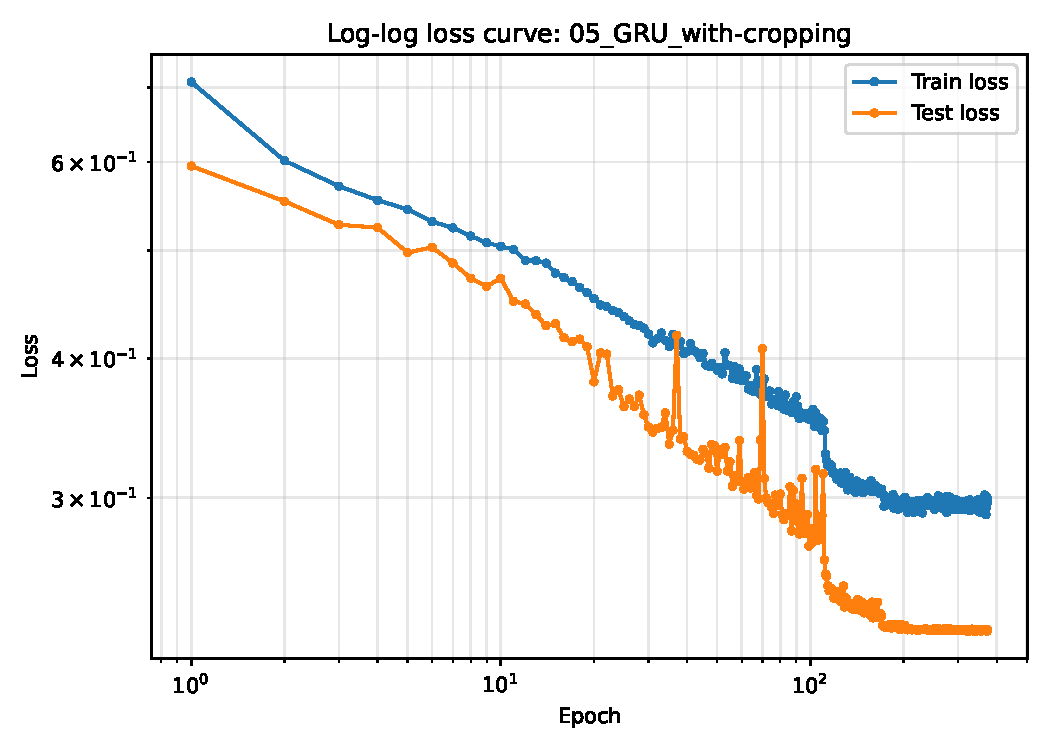
\includegraphics[width=\linewidth]{../figures/05_GRU_with-cropping_loss_curve_loglog}
  }

  \caption{Training and test loss as a function of epoch. The log-log representation makes both the rapid initial decrease and later convergence visible. Further loss curves can be found in the appendix (see Sec. \ref{sec:appendix}).}
  \label{fig:loss_curves}
\end{figure}

\subsection{Performance on Complete, Noise-Free Trajectories}

The velocity-only MLP achieves RMSE values of
$\SI{0.00640}{\meter\per\second}$,
$\SI{0.00677}{\meter\per\second}$, and
$\SI{0.00304}{\meter\per\second}$
for $v_x$, $v_y$, and $v_z$, respectively. This near-exact reconstruction is expected because its engineered inputs include a finite-difference estimate of the initial velocity. It should therefore be interpreted as a task-specific feature-engineering baseline rather than as evidence that the remaining physical parameters are equally identifiable.

Table \ref{tab:clean_results} compares representative outputs for the all-parameter models.
The MLP remains competitive for launch velocity, but the GRUs recover wind, spin direction, drag, and Magnus strength more accurately. Adding velocity and acceleration channels to the full-trajectory GRU reduces the RMSE of $u_x$ from
$\SI{2.67}{\meter\per\second}$ to $\SI{1.36}{\meter\per\second}$, of $\beta_D$ from
$\SI{0.00300}{\per\meter}$ to $\SI{0.00127}{\per\meter}$, and of $\beta_M$ from
$\SI{0.0378}{\per\second}$ to $\SI{0.0190}{\per\second}$.
The corresponding $R^2$ values increase from $0.899$ to $0.974$, from $0.920$ to $0.986$, and from $0.810$ to $0.952$, respectively.

\begin{table}[htbp]
    \centering
    \small
    \resizebox{\linewidth}{!}{%
    \begin{tabular}{lllll}
        \hline
        Target & MLP all & GRU positions & GRU derivatives & GRU cropped derivatives \\
        \hline
        $v_x\,[\si{\meter\per\second}]$
            & $1.016\;(0.998)$ & $1.793\;(0.995)$ & $1.027\;(0.998)$ & $1.223\;(0.998)$ \\
        $u_x\,[\si{\meter\per\second}]$
            & $3.857\;(0.789)$ & $2.667\;(0.899)$ & $1.359\;(0.974)$ & $1.413\;(0.972)$ \\
        $\omega_x$
            & $0.413\;(0.488)$ & $0.247\;(0.817)$ & $0.129\;(0.950)$ & $0.133\;(0.947)$ \\
        $\beta_D\,[\si{\per\meter}]$
            & $0.00445\;(0.825)$ & $0.00300\;(0.920)$ & $0.00127\;(0.986)$ & $0.00121\;(0.987)$ \\
        $\beta_M\,[\si{\per\second}]$
            & $0.0664\;(0.413)$ & $0.0378\;(0.810)$ & $0.0190\;(0.952)$ & $0.0191\;(0.952)$ \\
        \hline
    \end{tabular}}
    \caption{Per-target test performance on complete, noise-free trajectories. Each entry reports RMSE followed by $R^2$ in parentheses. Model names correspond to configurations 02, 03, 04, and 06 in Table~\ref{tab:model_configurations}.}
    \label{tab:clean_results}
\end{table}

Random-crop augmentation slightly sacrifices complete-trajectory accuracy for some outputs, but configuration 06 remains close to configuration 04. The endpoint-augmented derivative model likewise gives comparable parameter errors, for example $\operatorname{RMSE}(\beta_M)=\SI{0.0184}{\per\second}$.
Its endpoint MAEs are $\SI{1.22}{\meter}$ in $x$ and $\SI{1.17}{\meter}$ in $y$, while the corresponding RMSEs are $\SI{4.65}{\meter}$ and $\SI{3.35}{\meter}$. The gap between MAE and RMSE indicates that a minority of comparatively large endpoint errors remains. The auxiliary endpoint objective does not yield a consistent improvement of the $11$ physical-parameter predictions over configuration 06.

\subsection{Dependence on the Observed Trajectory Fraction}

Figure \ref{fig:cropping_performance} shows that GRUs trained only on complete trajectories deteriorate strongly when only an early prefix is available. Crop augmentation substantially reduces this distribution shift. For configuration 06 at $f=0.5$, the RMSEs are $\SI{1.08}{\meter\per\second}$ for $v_x$, $\SI{1.64}{\meter\per\second}$ for $u_x$, $0.150$ for $\omega_x$, $\SI{0.00136}{\per\meter}$ for $\beta_D$, and $\SI{0.0223}{\per\second}$ for $\beta_M$.
These values are close to the corresponding full-trajectory errors in Table \ref{tab:clean_results}. Even at $f=0.1$, configuration 06 yields $\operatorname{RMSE}(v_x)=\SI{2.16}{\meter\per\second}$, compared with $\SI{6.62}{\meter\per\second}$ for the derivative GRU trained only on complete trajectories. The remaining deterioration of wind, spin, and aerodynamic parameters at very small $f$ is physically plausible because these quantities influence curvature and deceleration over time, so their effects are only weakly expressed at the beginning of a flight.

\begin{figure}[htbp]
    \centering
    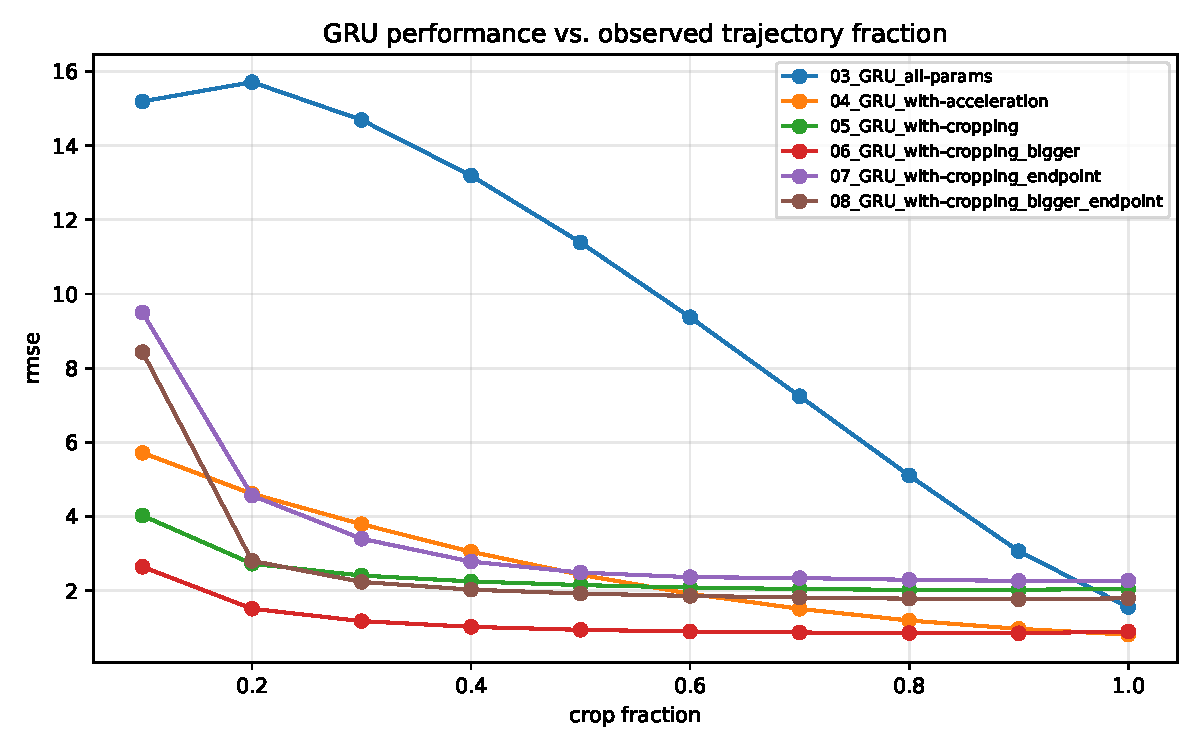
\includegraphics[width=0.92\linewidth]{../figures/gru_performance_vs_cropping.pdf}
    \caption{Diagnostic aggregate RMSE of the GRU configurations as a function of the observed trajectory fraction. Since the aggregate mixes outputs with different physical units, per-target values are used for quantitative interpretation.}
    \label{fig:cropping_performance}
\end{figure}

\subsection{Robustness to Gaussian Position Noise}

All GRUs are sensitive to measurement noise, and the degradation is already pronounced at $\sigma=\SI{0.01}{\meter}$, as shown in Figure \ref{fig:noise_performance}. For the derivative GRU without crop augmentation, the RMSE of $v_x$ increases from $\SI{1.03}{\meter\per\second}$ to $\SI{21.0}{\meter\per\second}$, while the RMSE of $u_x$ increases from $\SI{1.36}{\meter\per\second}$ to $\SI{9.50}{\meter\per\second}$. Over the same change, the $\beta_D$ error increases from $\SI{0.00127}{\per\meter}$ to $\SI{0.0120}{\per\meter}$. This behaviour is consistent with the fact that velocity and especially acceleration are obtained by differentiating already perturbed positions.

No single configuration dominates for every noisy target. At $\sigma=\SI{0.01}{\meter}$, the position-only endpoint model has a lower $v_x$ RMSE of $\SI{6.94}{\meter\per\second}$, but its $u_x$ RMSE is $\SI{20.3}{\meter\per\second}$, compared with $\SI{9.50}{\meter\per\second}$ for the derivative GRU. The results therefore reveal a trade-off between clean-data accuracy and target-dependent robustness. They also show that crop augmentation alone is not a substitute for noise augmentation: none of the training configurations adds Gaussian observation noise. A natural extension is to train with noise levels representative of the intended measurement system \cite{bishop1995training}, or to estimate derivatives using a smoothing or regularized procedure \cite{chartrand2011numerical}.

\begin{figure}[htbp]
    \centering
    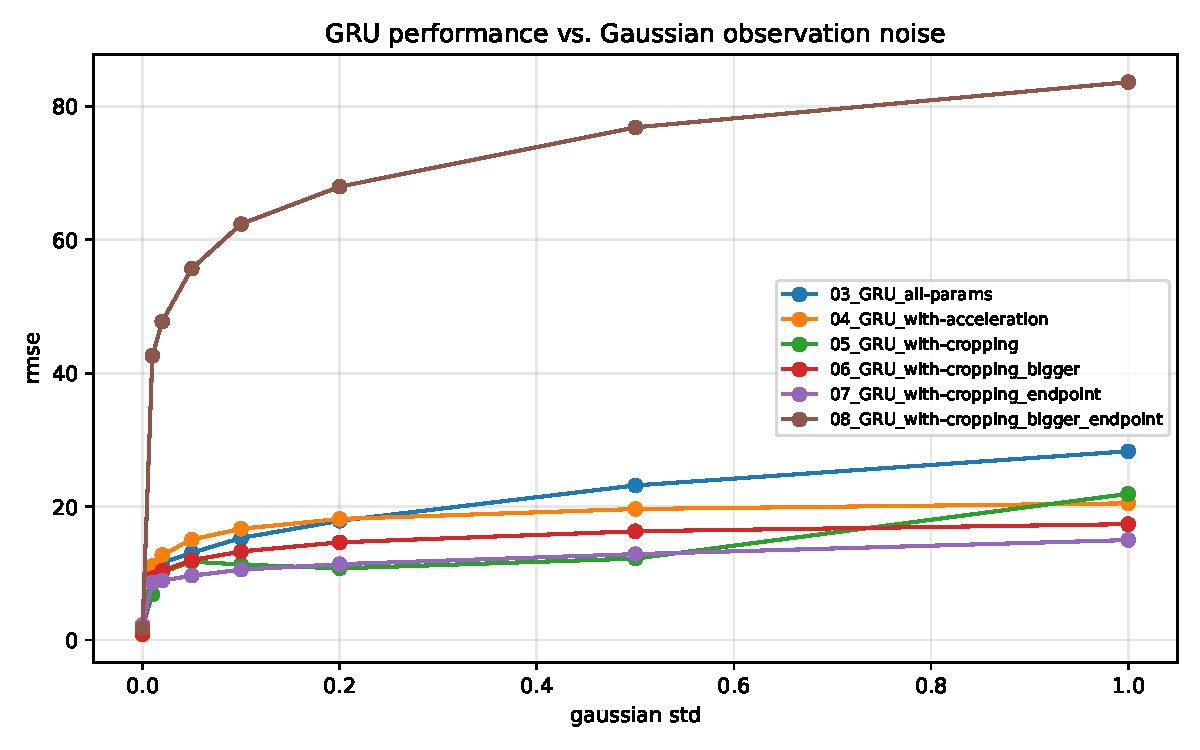
\includegraphics[width=0.92\linewidth]{../figures/gru_performance_vs_gaussian_noise.pdf}
    \caption{Diagnostic aggregate RMSE of the GRU configurations under independent Gaussian position noise. Noise is added before derivative features are computed. The aggregate curve is used qualitatively because it combines targets with different units.}
    \label{fig:noise_performance}
\end{figure}

Overall, engineered velocity features solve the restricted initial-velocity task extremely accurately, whereas sequence models are more effective for the joint inverse problem. For complete, clean trajectories, explicitly supplied derivatives provide the strongest overall parameter recovery. For partial trajectories, random-crop training is essential and retains useful accuracy down to substantially shorter prefixes. In contrast, the noise experiment exposes a major limitation of the present preprocessing pipeline: numerical derivatives improve clean-data accuracy but amplify positional noise.
